%!TEX encoding = UTF-8 Unicode
\documentclass{beamer}
\usepackage{amsmath,amsthm,amssymb}
\usepackage{CJKutf8}
\usepackage{graphicx}
\usepackage{hyperref}
\usepackage{pstricks-add}
\useoutertheme{sidebar}

\begin{document}
\begin{CJK}{UTF8}{bsmi}
\title{微積分的基石}
\subtitle{函數、極限、初等函數}
\author[何震邦]{何震邦 \href{http://jdh8.org/}{\textless jdh8.org\textgreater}\\
    \href{http://creativecommons.org/licenses/by-sa/3.0/tw/deed.zh\textunderscore TW}{\includegraphics{by-sa.eps}}}
\date{2012 年 10 月 17 日}
\maketitle

\begin{frame}{關於我}
  \begin{center}
    \includegraphics[width=0.3\textwidth]{sticker.eps}
  \end{center}
  \begin{itemize}
    \item \href{http://jdh8.org/}{jdh8.org}
    \item \href{mailto:jdh863@gmail.com}{jdh863@gmail.com}
    \item \href{http://www.facebook.com/jdh8.fr}{我的臉書}
    \item 0918-319823
      \begin{itemize}
	\item 真是充滿火藥味的號碼
      \end{itemize}
  \end{itemize}
\end{frame}

\section{函數}
\begin{frame}{函數就像射飛鏢}
  \begin{itemize}
    \item 飛鏢只有一個鏢頭,函數的值是唯一的
    \item 可以說函數是一種特殊的映射(mapping)
    \begin{itemize}
      \item 映射就沒有啥限制了,可以用霸王鏢
    \end{itemize}
  \end{itemize}
  \begin{center}
    \includegraphics[width=\textwidth]{invSqrt.ps}
  \end{center}
\end{frame}

\begin{frame}{誰規定函數只能有一個輸入值?}
  \begin{itemize}
    \item $\operatorname{add}(x,y) := x + y$
    \item $\operatorname{mul}(x,y) := xy$
    \item $\displaystyle \textup{B}(x,y) := \int_0^1 t^{x-1} (1-t)^{y-1} dt$
  \end{itemize}
\end{frame}

\subsection{函數的種類}
\begin{frame}{以函數的形式分類}
  \begin{itemize}
    \item 線性函數
    \item 多項式
    \item 有理函數
    \item 代數函數
    \item 初等函數
  \end{itemize}
\end{frame}

\begin{frame}{線性函數}
  \begin{definition}
    線性函數就是具有可加性與齊次性的函數
    \begin{align*}
      f(x + y) &= f(x) + f(y)\\
      f(cx) &= cf(x)
    \end{align*}
  \end{definition}
  \begin{itemize}
    \item 最簡單的例子,乘號!它是雙線性!
    \begin{itemize}
      \item 左邊也線性,右邊也線性,不就雙線性?
      \item 乘號不一定要有交換律噢!像外積跟矩陣乘積
    \end{itemize}
  \end{itemize}
\end{frame}

\begin{frame}{多項式}
  \begin{definition}
    \[f(x) = a_0 + a_1 x + \cdots + a_{n-1} x^{n-1} + a_n x^n = \sum_{i=0}^{n} a_i x^i\]
  \end{definition}
  \begin{itemize}
    \item 多項式可以表示為自變數與常數有限次的加、減、乘
    \item 多項式是平滑函數
    \begin{itemize}
      \item 平滑函數無窮可微
      \item 可微必連續
    \end{itemize}
  \end{itemize}
\end{frame}

\begin{frame}{有理函數}
  \begin{definition}
    \[f(x) = \frac{P(x)}{Q(x)}\]
    其中 $P$ 和 $Q$ 是多項式,且 $Q \ne 0$
  \end{definition}
  \begin{itemize}
    \item 有理函數可以表示為自變數與常數有限次的四則運算
    \item 在微積分上,我們常把有理函數分解成部份分式
      \begin{itemize}
	\item 微分跟積分都是線性算子
	\item 處理 $\dfrac{1}{ax + b}$ 比 $\dfrac{1}{ax^2 + bx + c}$ 容易多了!
      \end{itemize}
  \end{itemize}

  \[\frac{x^3 - 5x + 88}{x^2 + 3x - 28} = x-3 + \frac{32x + 4}{x^2 + 3x - 28} = x-3 + \frac{20}{x+7} + \frac{12}{x-4}\]
\end{frame}

\begin{frame}{代數函數}
  \begin{definition}
    代數函數 $y$ 是以下函數方程的解,其中係數 $a_i(x)$ 都是整係數多項式:
    \[a_n(x) y^n + a_{n-1}(x) y^{n-1} + \cdots + a_0(x) = 0\]
  \end{definition}
  \begin{itemize}
    \item 代數函數可以表示為自變數與常數有限次的加、減、乘、除和開方的運算(有理運算)
    \item $\sqrt{x^2 + 1}$ 是代數函數,但不是有理函數
  \end{itemize}
\end{frame}

\begin{frame}{初等函數}
  \begin{definition}
    初等函數是由冪函數($x^a$)、指數函數、對數函數、三角函數、反三角函數與常數經過有限次的有理運算和/或函數複合所產生
  \end{definition}
  \begin{itemize}
    \item 初等函數就是可以用解析式表示的函數
    \item $\lfloor x \rfloor$ 不是初等函數
    \item $\displaystyle erf(x) = \frac{2}{\sqrt\pi} \int_0^x e^{-t^2} dt$ 不是初等函數
    \item 但 $|x|$ 不小心在\textbf{實數}域上\textbf{是}初等函數(為什麼?)
  \end{itemize}
\end{frame}

\section{極限}
\begin{frame}{為什麼我們需要極限?}
  \begin{itemize}
    \item 我們很容易就能從自然數建構整數,再從整數建構有理數
    \item 接下來,人類學會建構代數數。代數數可以是整係數多項方程的解
    \item 但是有些不是代數數的數(超越數)就自動跑出來了,像是 $e$、$\pi$、$2^{\sqrt2}$ 等
    \item 對於這些數,我們如果要取值,只能用逼近的
  \end{itemize}
\end{frame}

\begin{frame}{正實數的實數冪}
  \begin{itemize}
    \item 正實數的有理次冪,可以用開方來獲得
    \item 但是 $2^{\sqrt2}$ 一定是開不出來的啦!
      \begin{itemize}
	\item 注意,證明做不出來,跟目前沒有人做出來,是不同的
	\item Lindermann--Weierstrass theorem: 如果 $\alpha$ 是非零代數數,則 $e^\alpha$ 是超越數
	\item Gelfond--Schneider theorem: 如果 $\alpha$ 和 $\beta$ 都是代數數,其中 $\alpha \ne 0$ 且 $\alpha \ne 1$,且 $\beta$
	    不是有理數,那麼 $\alpha^\beta$ 是超越數
      \end{itemize}
    \item 它的平方根 $\sqrt2^{\sqrt2}$ 也是一個超越數
      \begin{itemize}
	\item 無理數的無理數次方可以是有理數,如 $\left(\sqrt2^{\sqrt2}\right)^{\sqrt2}$
      \end{itemize}
    \item $\displaystyle 2^{\sqrt2} = \lim_{t\to\sqrt2} 2^t$
  \end{itemize}
\end{frame}

\subsection{極限與連續性}
\begin{frame}{極限的定義}
  \begin{definition}
    若對於所有正數 $\epsilon$,必存在一正數 $\delta$ 使得
    \[0 < |x-c| < \delta \Rightarrow |f(x) - L| < \epsilon\]
    則
    \[\lim_{x \to c} f(x) = L\]
  \end{definition}
\end{frame}

\begin{frame}{函數的連續性}
  \begin{definition}
    若函數 $f$ 在 $c$ 點連續,則符合以下條件
    \begin{itemize}
      \item $f(c)$ 有定義
      \item $\displaystyle \lim_{\mathbf x \to c} f(x)$ 存在
      \item $\displaystyle \lim_{\mathbf x \to c} f(x) = f(c)$
    \end{itemize}
  \end{definition}
\end{frame}

\subsection{$\epsilon$-$\delta$ 論證}
\begin{frame}{$\displaystyle \lim_{x \to c} r = r$}
  \begin{proof}
    \begin{enumerate}
      \item 若 $0 < |x-c| < \delta$ 則 $|r-r| = 0$
      \item 對於所有正數 $\epsilon$,存在 $\delta$ 使得若 $0 < |x-c| < \delta$ 則 $|r-r| = 0$
    \end{enumerate}
  \end{proof}
  \begin{center}
    \begin{pspicture}(0,0)(3,3)
      \newrgbcolor{Red}{1 0.7 0.7}
      \psframe*[linecolor=Red](0,0)(3,3)
      \psaxes(0,0)(3,3)
      \psline[linecolor=blue](0,1.5)(3,1.5)
    \end{pspicture}
  \end{center}
\end{frame}

\begin{frame}{$\displaystyle \lim_{x \to c} x = c$}
  \begin{proof}
    \begin{enumerate}
      \item 設 $\delta := \epsilon$
      \item 若 $0 < |x-c| < \delta$, 則 $|x-c| < \delta = \epsilon$
    \end{enumerate}
  \end{proof}
  \begin{center}
    \begin{pspicture}(0,0)(3,3)
      \newrgbcolor{Blue}   {0.7  0.7  1}
      \newrgbcolor{Red}    {1    0.7  0.7}
      \newrgbcolor{Magenta}{0.79 0.49 0.7}
      \psframe*[linecolor=Blue](0,1.25)(3,1.75)
      \psframe*[linecolor=Red](1.25,0)(1.75,3)
      \psframe*[linecolor=Magenta](1.25,1.25)(1.75,1.75)

      \psaxes(0,0)(3,3)
      \psline(0,0)(3,3)
      \psline[linecolor=blue](0,1.25)(3,1.25)
      \psline[linecolor=blue](0,1.75)(3,1.75)
      \psline[linecolor=red](1.25,0)(1.25,3)
      \psline[linecolor=red](1.75,0)(1.75,3)
    \end{pspicture}
  \end{center}
\end{frame}

\begin{frame}{$\displaystyle \lim_{x \to c} (f(x) + g(x)) = \lim_{x \to c} f(x) + \lim_{x \to c} g(x)$}
  \begin{proof}
    \begin{enumerate}
      \item 設 $\displaystyle L := \lim_{x \to c} f(x),\; M := \lim_{x \to c} g(x)$
      \item 設一任意正數 $\epsilon$,則我們有
	\begin{itemize}
	  \item 存在正數 $\delta_1$ 使得 $0 < |x-c| < \delta_1 \Rightarrow |f(x) - L| < \dfrac{\epsilon}{2}$
	  \item 存在正數 $\delta_2$ 使得 $0 < |x-c| < \delta_2 \Rightarrow |g(x) - M| < \dfrac{\epsilon}{2}$
	\end{itemize}
      \item 設 $\delta := \min(\delta_1, \delta_2)$,則
      \[|f(x) + g(x) - (L + M)| \le |f(x) - L| + |g(x) - M| < \frac{\epsilon}{2} + \frac{\epsilon}{2}\]
    \end{enumerate}
  \end{proof}
\end{frame}

\begin{frame}{$\displaystyle \lim_{x \to c} f(g(x)) = \lim_{u \to \lim_{x \to c} g(x)} f(u)$}
  \begin{proof}
    \begin{enumerate}
      \item 設 $\displaystyle M := \lim_{x \to c} g(x)$,並重新定義 $\displaystyle f(M) := \lim_{u \to M} f(u)$ 使 $f$ 在 $M$
	    上連續,不失一般性
      \item 設一任意正數 $\epsilon$
	\begin{itemize}
	  \item 存在正數 $\delta_1$ 使得 $0 < |u-M| < \delta_1 \Rightarrow |f(u) - f(M)| < \epsilon$
	  \item 當 $u = M$,我們也有 $f(u) = f(M)$ 即 $|f(u) - f(M)| = 0$
	  \item 存在正數 $\delta_1$ 使得 $|u-M| < \delta_1 \Rightarrow |f(u) - f(M)| < \epsilon$
	\end{itemize}
      \item 設 $\epsilon_1 := \delta_1$
	\begin{itemize}
	  \item 存在正數 $\delta$ 使得 $0 < |x-c| < \delta \Rightarrow |g(x) - M| < \epsilon_1$
	  \item 若 $|g(x) - M| < \delta_1$ 則 $|f(g(x)) - f(M)| < \epsilon$
	\end{itemize}
      \item 所以 $\displaystyle \lim_{x \to c} f(g(x)) = f(M) = \lim_{u \to M} f(u)$
    \end{enumerate}
  \end{proof}
\end{frame}

\subsection{極限的運算}
\begin{frame}{初等函數在定義域上連續}
  \begin{itemize}
    \item 只有以上四個命題需要使用 $\epsilon$-$\delta$ 論述證明
    \item 連續函數的反函數也連續
      \[\lim_{u \to \lim_{x \to c} f(x)} f^{-1}(u) = \lim_{x \to c} f^{-1}(f(x)) = \lim_{x \to c} x = c\]
    \item 代數函數、冪函數、指數函數都可以用常數、變數、加法、複合函數、反函數這五者組合出來
    \item 下次我們將證明三角函數也在定義域上連續
  \end{itemize}
\end{frame}

\begin{frame}{多項式是連續函數}
  \[\lim_{x \to c} (f(x) - g(x)) = \lim_{x \to c} f(x) - \lim_{x \to c} g(x)\]
  \begin{align*}
    \lim_{x \to c} k f(x) &= k \lim_{x \to c} f(x)                               &k \in \mathbb Z\\
    \lim_{x \to c} \frac{f(x)}{n} &= \frac{\displaystyle \lim_{x \to c} f(x)}{n} &n \in \mathbb N\\
    \lim_{x \to c} b f(x) &= b \lim_{x \to c} f(x)                               &b \in \mathbb Q\\
    \lim_{x \to c} a f(x) &= \lim_{x \to c} \left(\left( \lim_{b \to a} b \right) f(x) \right) = a \lim_{x \to c} f(x)
      &b \in \mathbb Q\\
  \end{align*}
  \[\lim_{x \to c} f(\left. x \right) g(x) = \lim_{x \to c} \left( f(x) \lim_{x \to c} g(x) \right)
      = \lim_{x \to c} f(x) \lim_{x \to c} g(x)\]
\end{frame}

\begin{frame}{初等函數在定義域上連續}
  \begin{align*}
    \lim_{x \to c} \frac{f(x)}{g(x)}
	&= \frac{\displaystyle \lim_{x \to c} f(x)}{\displaystyle \lim_{x \to c} g(x)} &g(x) \ne 0\\
    \lim_{x \to c} f(x)^k &= \left( \lim_{x \to c} f(x) \right)^k                      &k \in \mathbb Z,\; f(x) \ne 0\\
    \lim_{x \to c} \sqrt[n]{f(x)} &= \sqrt[n]{\displaystyle \lim_{x \to c} f(x)}       &n \in \mathbb N,\; f(x) > 0\\
    \lim_{x \to c} f(x)^b &= \left( \lim_{x \to c} f(x) \right)^b                      &b \in \mathbb Q,\; f(x) > 0\\
    \lim_{x \to c} f(x)^a      &= \left( \lim_{x \to c} f(x) \right)^a      &f(x) > 0\\
    \lim_{x \to c} f(x)^{g(x)} &= \left( \lim_{x \to c} f(x) \right)^{g(x)} &f(x) > 0
  \end{align*}
\end{frame}

\subsection{無窮極限、單邊極限}
\begin{frame}{無窮極限}
  \begin{definition}
    若對於所有正數 $r$,均能找到一正數 $\delta$ 使得 $0 < |x-c| < \delta \Rightarrow f(c) > r$,則
    \[\lim_{x \to c} f(x) = \infty\]
    若對於所有負數 $r$,均能找到一正數 $\delta$ 使得 $0 < |x-c| < \delta \Rightarrow f(c) < r$,則
    \[lim_{x \to c} f(x) = -\infty\]
  \end{definition}
  \begin{itemize}
    \item $\infty$ 就是比任何一個實數都大!
  \end{itemize}
\end{frame}

\begin{frame}{單邊極限}
  \begin{definition}
    若對於所有正數 $\epsilon$,均能找到一正數 $\delta$ 使得 $c < x < c + \delta \Rightarrow |f(c) - L| < \epsilon$,則
    \[\lim_{x \to c^+} f(x) = L\]
    若對於所有正數 $\epsilon$,均能找到一正數 $\delta$ 使得 $c - \delta < x < c \Rightarrow |f(c) - L| < \epsilon$,則
    \[\lim_{x \to c^-} f(x) = L\]
  \end{definition}
  \begin{itemize}
    \item 先前我們觀察的區間是 $0 < |x-c| < \delta$,所是會觀察到 $x$ 在 $c$ 兩側的行為
    \item 如果只觀察 $0 < x-c < \delta$,就只會觀察到右側,反之亦然。
  \end{itemize}
\end{frame}

\section{初等函數}
\begin{frame}{複習初等函數}
  \begin{itemize}
    \item 在高中的時候,我們已經把初等函數學得差不多了,除了
      \begin{itemize}
	\item 自然指數、自然對數
	\item 反三角函數
      \end{itemize}
  \end{itemize}
\end{frame}

\subsection{指數與對數}
\begin{frame}{指數函數}
  \begin{itemize}
    \item 有理數具有稠密性,所以我們可以用有理數列來逼近一個無理數,像這樣
    \[\lim_{b \to r} b = r,\; b \in \mathbb Q,\; r \in \mathbb R\]
    \item 自然指數就是以 e 為底的指數函數,其中
    \[\textup e := \lim_{n\to\infty} \left(1 + \frac{1}{n}\right)^n \approx 2.718281828\]
    \begin{itemize}
      \item 這個數列的收斂速度非常慢,到了第 $n$ 項大概只有 $\log n$ 位的有效位數
      \item 我們有更有效的方法來計算 $\textup e^x$
    \end{itemize}
  \end{itemize}
\end{frame}

\begin{frame}{$\textup e^x$ 的圖形}
  \begin{center}
    \begin{pspicture}(-4,0)(4,5)
      \psaxes(0,0)(-4,0)(4,5)
      \psplot[plotstyle=curve]{-4}{1.609437912}{x EXP}
      \psline[linestyle=dashed](-1.15,-0.15)(4,5)
    \end{pspicture}
  \end{center}
\end{frame}

\begin{frame}{對數函數}
  \begin{itemize}
    \item 人類是先有對數才有指數!
    \item 不過就現代數學而言,通常把 $\log_b x$ 定義為 $b^x$ 的反函數。其中 $\ln := \log_{\textup e}$
    \item 為什麼要拿這麼奇怪的數字當底數呢?
  \end{itemize}
\end{frame}

\begin{frame}{自然對數}
  \begin{itemize}
    \item 在沒有計算機的年代,算乘法是大工程
      \begin{itemize}
	\item $n$ 位數加法的時間複雜度:$O(n)$
	\item $n$ 位數\textbf{直式}的乘法的時間複雜度:$O(n^2)$
      \end{itemize}
    \item 對數表可以把乘法映射(map)到加法,加完再用反對數映射回去
    \item 對數表要怎麼製作呢?
      \begin{itemize}
	\item 乘方比開方好算
	\item 算 $x^n$ 頂多只要 $2 \log_2 n$ 次乘法(不是 $n-1$?)
	\item 底數要小到接近 1 才能避免開方
      \end{itemize}
  \end{itemize}
\end{frame}

\begin{frame}{納皮爾對數}
  \begin{itemize}
    \item 納皮爾(John Napier,1550--1617)先以 $\displaystyle\left(1 + \frac{1}{10^7}\right)$ 為底算出對數值,再把結果除以
	$10^7$。也就是製作以 $\displaystyle\left(1 + \frac{1}{10^7}\right)^{10^7}$ 為底的對數表
    \item 當後來要求的精度越來越精確,我們逐步把 $10^7$ 提升到更高的數字,最後乾脆取極限
  \end{itemize}
  \[\textup e := \lim_{n\to\infty} \left(1 + \frac{1}{n}\right)^n\]
\end{frame}

\subsection{三角函數}
\begin{frame}{三角函數的定義}
  \begin{center}
    \psset{unit=0.375\textwidth}
    \begin{pspicture}(0,0)(2.3662016,1)
      \psarc[linecolor=gray](0,0){1}{0}{90}
      \psarc(0,0){0.1}{0}{65}\rput[l](0.1,0.1){$\theta$}
      \psline[linecolor=gray](0,0)(0.42261826,0.90630779)
      \psline{->}(0.42261826,0)(0.42261826,0.90630779)\rput[l](0.47261826,0.45315389){sin}
      \psline{->}(0,0.90630779)(0.42261826,0.90630779)\rput[t](0.21130913,0.85630779){cos}
      \psline{->}(0.42261826,0.90630779)(2.3662016,0)\rput[l](1.1831008,0.75){tan}
      \psline{->}(0.42261826,0.90630779)(0,1.1033779)\rput[b](0.21130913,1.1){cot}
      \psline{->}(0,0)(2.3662016,0)\rput[t](1.1831008,-0.05){sec}
      \psline{->}(0,0)(0,1.1033779)\rput[r](-0.05,0.55168896){csc}
    \end{pspicture}
  \end{center}
\end{frame}

\begin{frame}{三角函數的性質}
  \begin{center}
    \psset{unit=0.1\textwidth,yunit=1.7320508}
    \begin{pspicture}(-2,-1.3)(2,1.3)
      \pspolygon[fillcolor=gray,fillstyle=solid](0,0)(1,1)(-1,1)
      \pspolygon[fillcolor=gray,fillstyle=solid](0,0)(-2,0)(-1,-1)
      \pspolygon[fillcolor=gray,fillstyle=solid](0,0)(2,0)(1,-1)
      \psline(-1,1)(-2,0)\psline(1,1)(2,0)\psline(-1,-1)(1,-1)
      \pscircle[fillcolor=white,fillstyle=solid](0,0){0.5}\rput(0,0){1}
      \pscircle[fillcolor=white,fillstyle=solid](-1,1){0.5}\rput(-1,1){sin}
      \pscircle[fillcolor=white,fillstyle=solid](1,1){0.5}\rput(1,1){cos}
      \pscircle[fillcolor=white,fillstyle=solid](-2,0){0.5}\rput(-2,0){tan}
      \pscircle[fillcolor=white,fillstyle=solid](2,0){0.5}\rput(2,0){cot}
      \pscircle[fillcolor=white,fillstyle=solid](-1,-1){0.5}\rput(-1,-1){sec}
      \pscircle[fillcolor=white,fillstyle=solid](1,-1){0.5}\rput(1,-1){csc}
    \end{pspicture}
  \end{center}
\end{frame}

\begin{frame}{餘弦差角公式}
  \begin{center}
    \psset{unit=0.2\textwidth}
    \begin{pspicture}(-1,-1)(1,1)
      \psaxes[labels=none](0,0)(-1,-1)(1,1)
      \pscircle[linecolor=gray](0,0){1}
      \psarc(0,0){0.2}{0}{28.647890}\uput[0](0.25,0.1){$\beta$}
      \psarc(0,0){0.1}{28.647890}{114.59156}\uput[90](0.1,0.1){$\alpha-\beta$}
      \psdots(0.87758256,0.47942554)(-0.41614684,0.90929743)
      \rput[b](-0.46614684,0.95929743){$A(\cos\alpha,\sin\alpha)$}
      \rput[l](0.92758256,0.52942554){$B(\cos\beta,\sin\beta)$}
      \pspolygon(0,0)(0.87758256,0.47942554)(-0.41614684,0.90929743)
    \end{pspicture}
  \end{center}
  \begin{align*}
    \overline{AB}^2 &= (\cos\alpha-\cos\beta)^2 + (\sin\alpha-\sin\beta)^2\\
		    &= 2 - 2(\cos\alpha\cos\beta + \sin\alpha\sin\beta)\\
    \overline{AB}^2 &= 1 + 1 - 2\cdot1\cdot1\cdot\cos(\alpha-\beta) = 2 - 2\cos(\alpha-\beta)\\
    \cos(\alpha-\beta) &= \cos\alpha\cos\beta + \sin\alpha\sin\beta
  \end{align*}
\end{frame}

\begin{frame}{反三角函數}
  \begin{itemize}
    \item Wait! 每個三角函數都有 $2\pi$ 這個週期,所以鐵定不是一對一函數啊!怎麼會有反函數咧?
    \item 我們可以把他們限制在一個區間內,讓他在區間內是一對一函數
      \begin{itemize}
	\item 為了方便,我們會讓區間包含 0 和 1,讓數字看起來比較舒服
      \end{itemize}
  \end{itemize}
  \begin{center}
    \begin{tabular}{lll}
      函數    & 受限的定義域              & 值域\\\hline
      $\sin x$& $[-\frac{\pi}{2},\frac{\pi}{2}]$          & $[-1,1]$\\
      $\cos x$& $[0,\pi]$                                 & $[-1,1]$\\
      $\tan x$& $(-\frac{\pi}{2},\frac{\pi}{2})$          & $\mathbb R$\\
      $\cot x$& $(0,\pi)$                                 & $\mathbb R$\\
      $\sec x$& $[0,\frac{\pi}{2})\cup(\frac{\pi}{2},\pi]$& $(-\infty,-1]\cup[1,\infty)$\\
      $\csc x$& $[-\frac{\pi}{2},0)\cup(0,\frac{\pi}{2}]$ & $(-\infty,-1]\cup[1,\infty)$
    \end{tabular}
  \end{center}
\end{frame}

\begin{frame}{謝謝聆聽!}
  \begin{center}
    \includegraphics[width=0.3\textheight]{favicon}
  \end{center}
  \begin{itemize}
    \item \href{http://jdh8.org/}{部落格}
    \item \href{http://boards.jdh8.org/cal/}{討論版}
    \item \href{https://github.com/jdh8/calculus-2012}{系列教材}
  \end{itemize}
\end{frame}

\end{CJK}
\end{document}
